\documentclass[titlepage,11pt]{article}
\usepackage{comment}
\usepackage[utf8]{inputenc} 
\usepackage[T1]{fontenc}  
\usepackage{enumitem}
\usepackage{transparent} % Untuk transparansi gambar
\usepackage{listings}
\usepackage{amsmath}
\usepackage{amsfonts}          % Font matematika
\usepackage{amssymb}
\usepackage{graphicx}
\usepackage[font=small,labelfont=bf]{caption}
\usepackage[bahasa]{babel}
\usepackage{float}
\usepackage{array}
\usepackage{verbatim}
\usepackage{listings}          % Untuk menampilkan kode (alternatif dari verbatim)
\usepackage{enumitem} 
\usepackage{graphicx,tabularx,multirow}
\usepackage{xcolor}
\usepackage[onehalfspacing]{setspace}
\usepackage[
	allcolors=visigrey,
	colorlinks=true,
]{hyperref}
\usepackage[a4paper,left=2cm,right=2cm]{geometry}
% Pengaturan kutipan artikel
\usepackage[style=ieee, backend=biber]{biblatex}
%Code listing style pak akok
\definecolor{codegreen}{rgb}{0,0.6,0}
\definecolor{codegray}{rgb}{0.5,0.5,0.5}
\definecolor{codepurple}{rgb}{0.58,0,0.82}
\definecolor{backcolour}{rgb}{0.95,0.95,0.92}

\usepackage{eso-pic} % Untuk menambahkan elemen ke seluruh halaman

\newcommand\BackgroundPic{
  \put(0,0){
    \parbox[b][\paperheight]{\paperwidth}{
      \vfill
      \centering
      \transparent{0.1}
      
\includegraphics[width=0.4\paperwidth,keepaspectratio]{miot.png}
      \vfill
    }
  }
}

\newcommand\BackgroundAllPages{ \AddToShipoutPicture*{\BackgroundPic} }
\newcommand\BackgroundNone{ \ClearShipoutPicture } % hilangkan background

\lstdefinestyle{mystyle}{
	backgroundcolor=\color{backcolour}, commentstyle=\color{codegreen},
	keywordstyle=\color{magenta},
	numberstyle=\small\color{codegray},
	stringstyle=\color{codepurple},
	basicstyle=\ttfamily\footnotesize,
	breakatwhitespace=false,         
	breaklines=true,                 
	captionpos=t,                    
	keepspaces=true,                 
	numbers=left,                    
	numbersep=5pt,                  
	showspaces=false,                
	showstringspaces=false,
	showtabs=false,           
	frame = single,
	tabsize=2
}
\lstset{style=mystyle}

\definecolor{visigrey}{rgb}{.1,.15,.15}
\geometry{top=1cm,bottom=.5cm}
\savegeometry{titlepage}
\geometry{top=2cm,bottom=2cm}
\savegeometry{main}

\def\bspace{\(\qquad\qquad\qquad\)}
\usepackage[T1]{fontenc}
\usepackage[utf8]{inputenc}
\usepackage{tgheros}
\renewcommand*\familydefault{\sfdefault}

\setcounter{tocdepth}{6}

\def\autor{Laboratorium }
\def\lab{Multimedia dan Internet of Things}
\def\departemen{Departemen Teknik Komputer}
\def\institut{Institut Teknologi Sepuluh Nopember}
\def\praktikum{Laporan Sementara \\ Praktikum Jaringan Komputer}
\def\nama{Abraham Napitupulu - 5024231048}
% Ubah Judul sesuai dengan modul
\def\judul{Tunneling}
\def\tanggal{2025}
\begin{document}
% Ubah Bahasa sesuai dengan keinginan
\selectlanguage{bahasa}

\BackgroundNone
\def\headingtype{\bf \small}
\loadgeometry{titlepage}

\begin{titlepage}
	\centering
	\begin{tabularx}{\textwidth}{l@{\hskip 0pt}lX}
		\raisebox{-0.5\height}{
\includegraphics[width=3cm]{Cover/img/logodepart.png}} 
		& \raisebox{-0.5\height}{
\includegraphics[width=3cm]{Cover/img/miot.png}} 
		& \raggedleft
	\hfill
	\begin{minipage}{0.5\textwidth}
		\raggedleft
		{\emph{\headingtype \autor}} \\[-2pt]
		{\headingtype \lab} \\[-2pt]
		{\headingtype \departemen} \\[-2pt]
		{\headingtype \emph{\institut}}
	\end{minipage}

	\vspace{5cm}
	\end{tabularx}
	
	\vspace{5cm}
	{\Huge \bf \praktikum \par}
	
	\vspace{2cm}
	{\LARGE \bf \judul \par}
	
	\vspace{2cm}
	{\Large \nama \par}
	
	\vfill
	{\Large \tanggal \par}
	
	\vfill
	
\includegraphics[width=\textwidth]{Cover/img/footer.png}
\end{titlepage}

\loadgeometry{main}


\BackgroundAllPages
% Pilih Modul yang akan di build
\section*{Laporan Hasil Percobaan Tunneling \& QoS}
\addcontentsline{toc}{section}{Laporan Hasil Percobaan Tunneling \& QoS}

\section{Langkah-Langkah Percobaan}
\addcontentsline{toc}{section}{Langkah-Langkah Percobaan}
Pada praktikum ini, saya melakukan dua skenario konfigurasi utama pada router MikroTik. Skenario pertama adalah membangun sebuah server VPN (Virtual Private Network) menggunakan protokol PPTP untuk memungkinkan akses jarak jauh yang aman. Skenario kedua adalah mengimplementasikan Quality of Service (QoS) untuk manajemen bandwidth menggunakan Simple Queue.

\subsection*{$\bullet$ Konfigurasi VPN PPTP (Remote Access)}
\addcontentsline{toc}{subsection}{Konfigurasi VPN PPTP (Remote Access)}
Proses ini bertujuan untuk membuat router berfungsi sebagai server PPTP, sehingga klien dari jaringan luar dapat terhubung ke jaringan lokal router.

\begin{enumerate}
    \item \textbf{Reset dan Login Router:} Langkah awal adalah mereset router ke konfigurasi pabrik tanpa pengaturan default untuk memastikan tidak ada konflik. Setelah itu, saya login kembali menggunakan Winbox via MAC Address dengan username \texttt{admin} dan password kosong.
    
    \item \textbf{Konfigurasi DHCP Client:} Saya mengkonfigurasi \texttt{ether3} sebagai DHCP Client agar router mendapatkan alamat IP dan koneksi dari sumber internet (ISP). Opsi \textit{Use Peer DNS} dan \textit{Use Peer NTP} dipastikan aktif.
    \begin{center}
        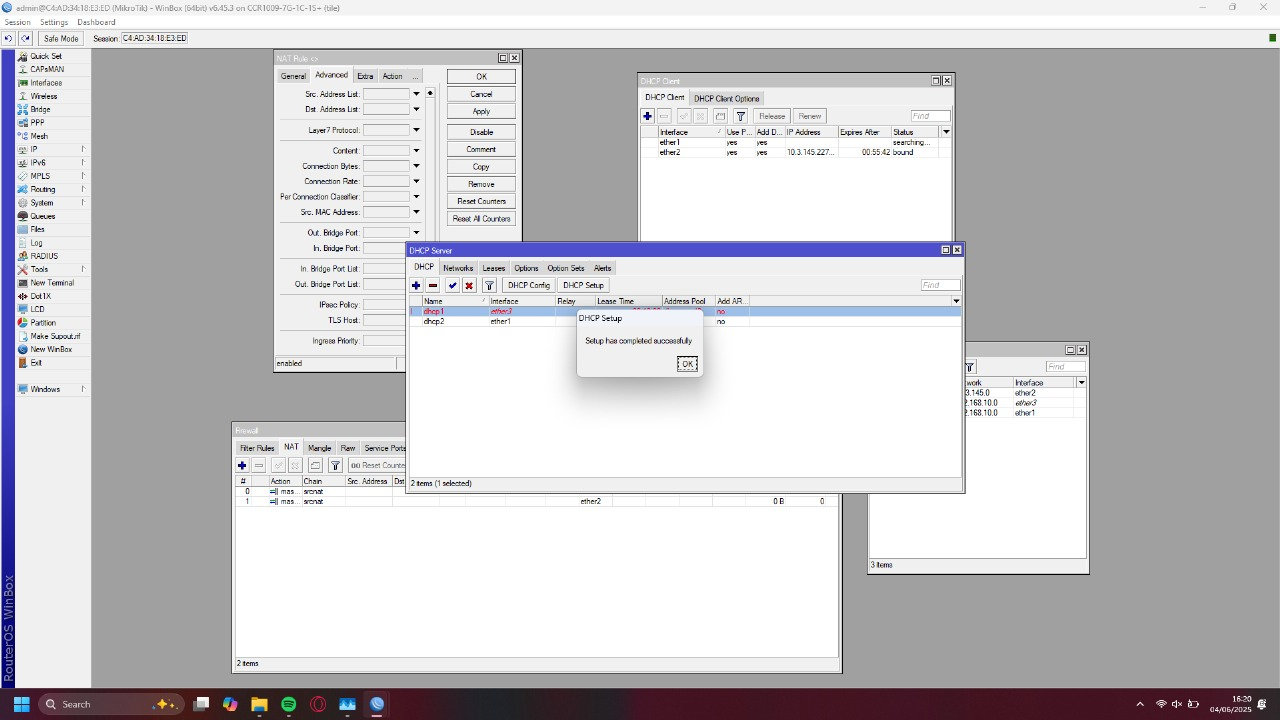
\includegraphics[width=0.7\textwidth]{img5/DHCPClient.jpeg} 
        \captionof{figure}{Konfigurasi DHCP Client pada antarmuka ether3.}
    \end{center}
    
    \item \textbf{Konfigurasi Firewall NAT:} Aturan NAT \textbf{masquerade} saya terapkan pada \textit{chain} \texttt{srcnat} dengan \textit{Out. Interface} mengarah ke \texttt{ether3}. Ini adalah langkah krusial agar semua perangkat di jaringan lokal nantinya bisa mengakses internet.
    
    \item \textbf{Konfigurasi IP Address LAN:} Saya menambahkan alamat IP statis \texttt{192.168.10.2/24} ke antarmuka \texttt{ether1} yang akan berfungsi sebagai gateway untuk jaringan lokal.
    \begin{center}
        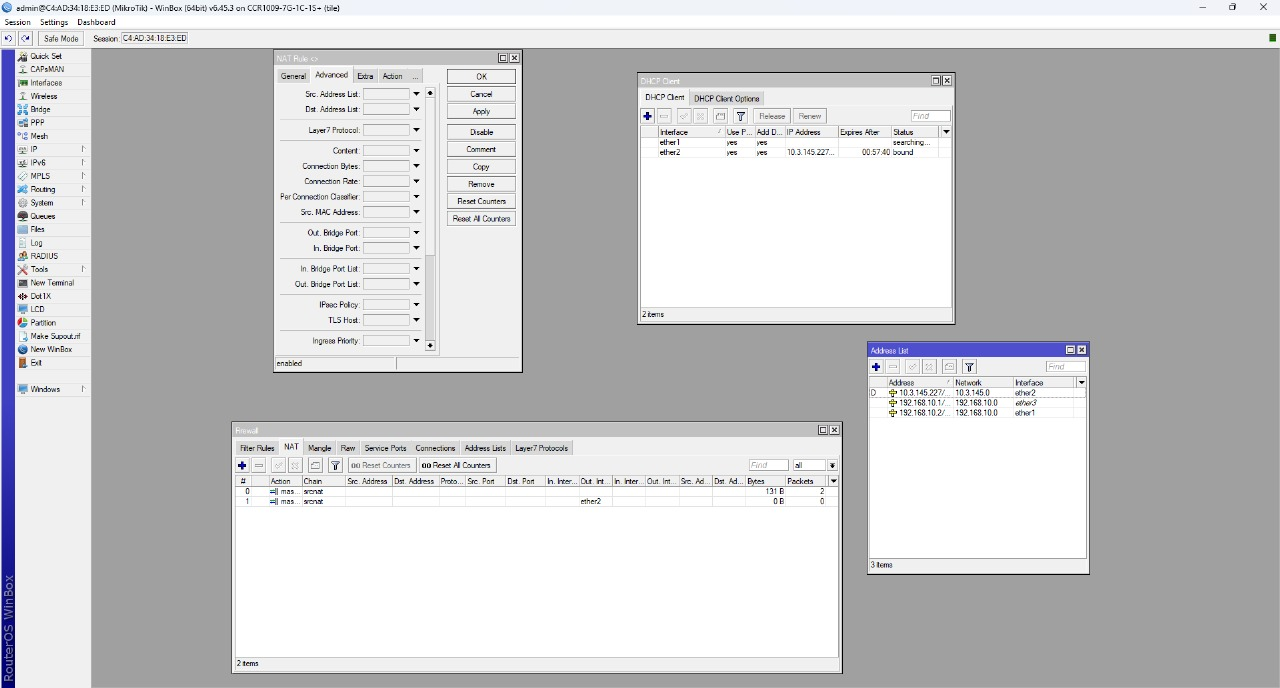
\includegraphics[width=0.7\textwidth]{img5/LANIP.jpeg} 
        \captionof{figure}{Penambahan alamat IP untuk jaringan lokal pada ether1.}
    \end{center}
    
    \item \textbf{Konfigurasi DHCP Server:} Melalui wizard \textit{DHCP Setup}, saya mengkonfigurasi DHCP Server pada antarmuka \texttt{ether1} untuk mendistribusikan IP ke klien. Sesuai modul, \textit{Gateway for DHCP Network} diatur ke \texttt{192.168.10.2}.
    
    \item \textbf{Mengaktifkan Proxy ARP:} Pada pengaturan antarmuka \texttt{ether1}, mode ARP saya ubah dari \textit{enabled} menjadi \textbf{proxy-arp} untuk membantu proses routing dan bridging pada koneksi VPN.
    
    \item \textbf{Mengaktifkan PPTP Server:}
    \begin{enumerate}[label*=\alph*.]
        \item Melalui menu \textit{PPP}, saya membuka jendela \textit{PPTP Server} dan mencentang kotak \textbf{Enabled}.
        \item Selanjutnya, saya membuat kredensial login pada tab \textit{Secrets} dengan detail sebagai berikut: \textit{Name}: \texttt{mahasiswa}, \textit{Password}: \texttt{praktikum123}, \textit{Service}: \texttt{pptp}, \textit{Local Address}: \texttt{192.168.10.2}, dan \textit{Remote Address}: \texttt{192.168.10.5}.
    \end{enumerate}
    \begin{center}
        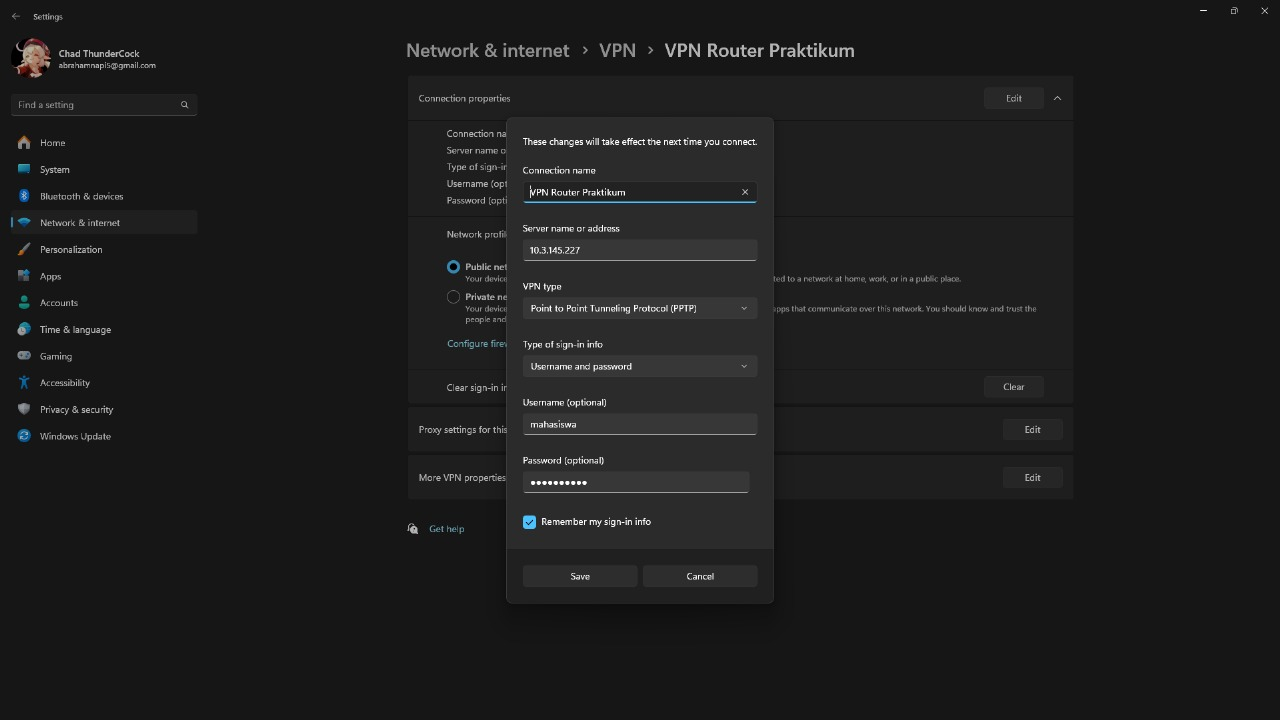
\includegraphics[width=0.7\textwidth]{img5/PPTPSecret.jpeg} 
        \captionof{figure}{Pembuatan user dan password untuk klien VPN pada tab Secrets.}
    \end{center}
    
    \item \textbf{Konfigurasi PPTP Client di Windows:} Saya menambahkan koneksi VPN baru di laptop Windows, mengisikan nama koneksi, alamat server (IP publik router di \texttt{ether3}), tipe VPN (PPTP), serta username dan password yang telah dibuat pada langkah sebelumnya.
    
    \item \textbf{Pengujian Koneksi VPN:} Setelah terhubung ke VPN, saya melakukan verifikasi.
    \begin{enumerate}[label*=\alph*.]
        \item Uji \texttt{ipconfig} di CMD laptop menunjukkan adanya antarmuka PPP baru dengan IP \texttt{192.168.10.5}.
        \item Uji \texttt{ping} dari laptop (klien VPN) ke gateway tunnel (\texttt{192.168.10.2}) berhasil.
        \item Uji \texttt{ping} dari laptop (klien VPN) ke PC lain di jaringan lokal (\texttt{ether1}) juga berhasil, menandakan tunnel telah berfungsi dengan baik.
    \end{enumerate}
    \begin{center}
        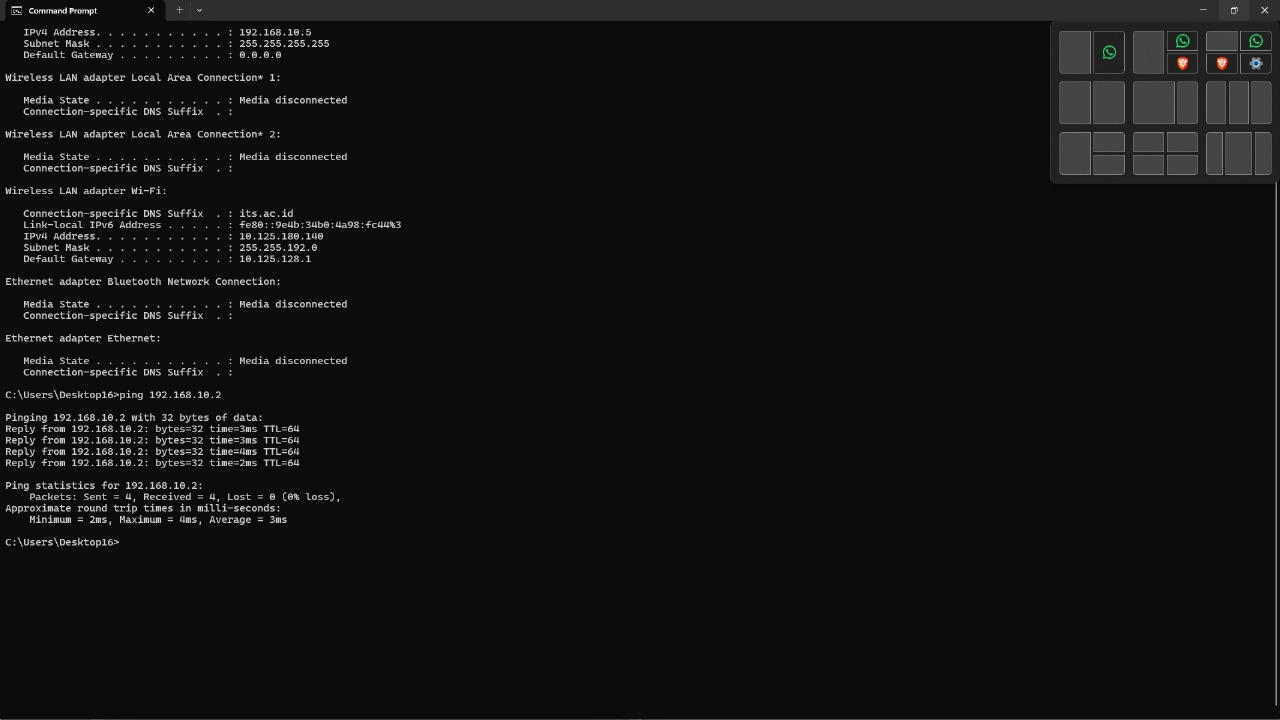
\includegraphics[width=0.7\textwidth]{img5/VPNTestping.jpeg} 
        \captionof{figure}{Hasil uji ping yang berhasil dari klien VPN ke gateway lokal.}
    \end{center}
\end{enumerate}

\subsection*{$\bullet$ Konfigurasi QoS dengan Simple Queue}
\addcontentsline{toc}{subsection}{Konfigurasi QoS dengan Simple Queue}
Skenario ini bertujuan untuk membatasi kecepatan internet untuk klien di jaringan lokal menggunakan fitur Simple Queue. Konfigurasi ini dilakukan tanpa mereset router dari skenario sebelumnya.

\begin{enumerate}
    \item \textbf{Membuat Aturan Simple Queue:}
    \begin{enumerate}[label*=\alph*.]
        \item Saya mengakses menu \textit{Queues}, lalu pada tab \textit{Simple Queues}, saya klik ikon `+`.
        \item Saya menamai queue \texttt{Limit-PC-Klien}.
        \item Pada kolom \textit{Target}, saya memasukkan network LAN: \texttt{192.168.10.0/24}.
        \item \textit{Max Limit} untuk Upload dan Download saya atur ke \textbf{1M} (1 Mbps).
    \end{enumerate}
    \begin{center}
        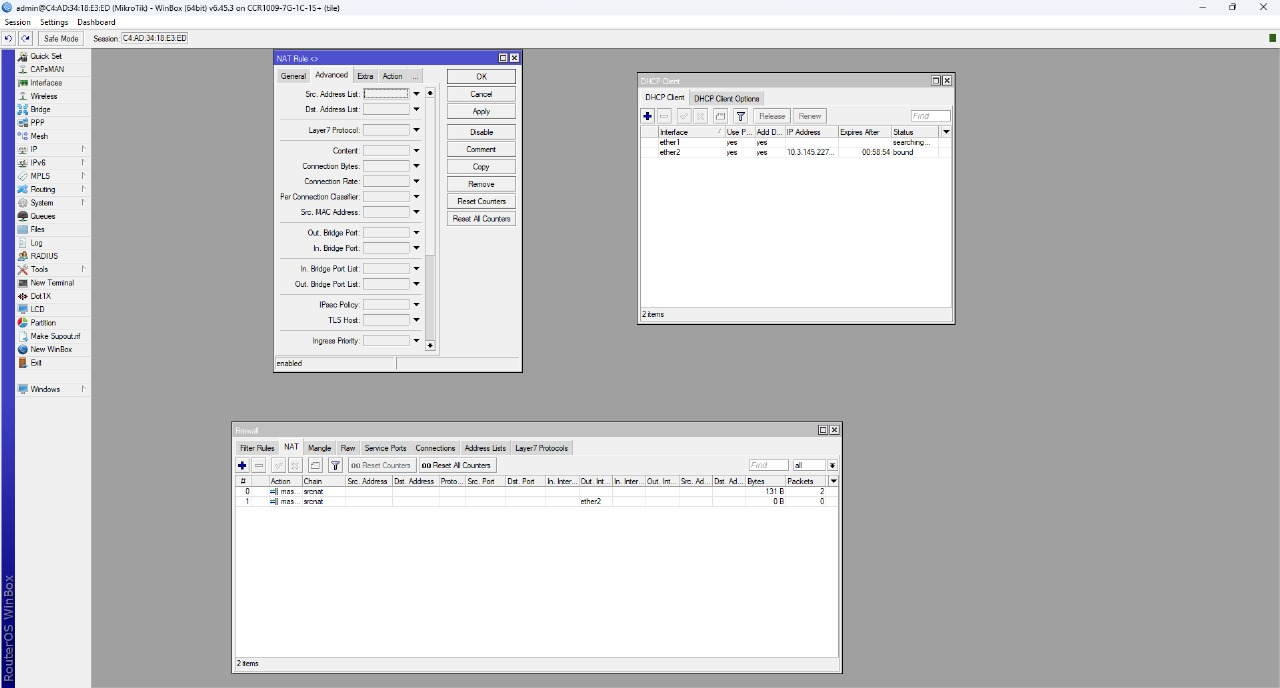
\includegraphics[width=0.7\textwidth]{img5/SimpleQ.jpeg} 
        \captionof{figure}{Pengaturan Simple Queue untuk membatasi bandwidth jaringan lokal.}
    \end{center}
    
    \item \textbf{Pemantauan Trafik:} Saya membuka kembali aturan queue tersebut dan pindah ke tab \textit{Traffic} untuk melihat grafik penggunaan bandwidth secara real-time.
    
    \item \textbf{Pengujian Efektivitas Queue:} Saya melakukan pengujian kecepatan internet dari PC klien dalam dua kondisi.
    \begin{enumerate}[label*=\alph*.]
        \item \textbf{Saat Queue Tidak Aktif:} Saya menonaktifkan aturan queue dan menjalankan speed test. Hasilnya menunjukkan kecepatan maksimal yang didapat dari ISP.
        \item \textbf{Saat Queue Aktif:} Saya mengaktifkan kembali aturan queue dan menjalankan speed test lagi. Hasilnya menunjukkan kecepatan upload dan download sekarang terbatas di sekitar 1 Mbps.
    \end{enumerate}
     \begin{figure}[H]
        \centering
        \begin{minipage}{0.48\textwidth}
            \centering
            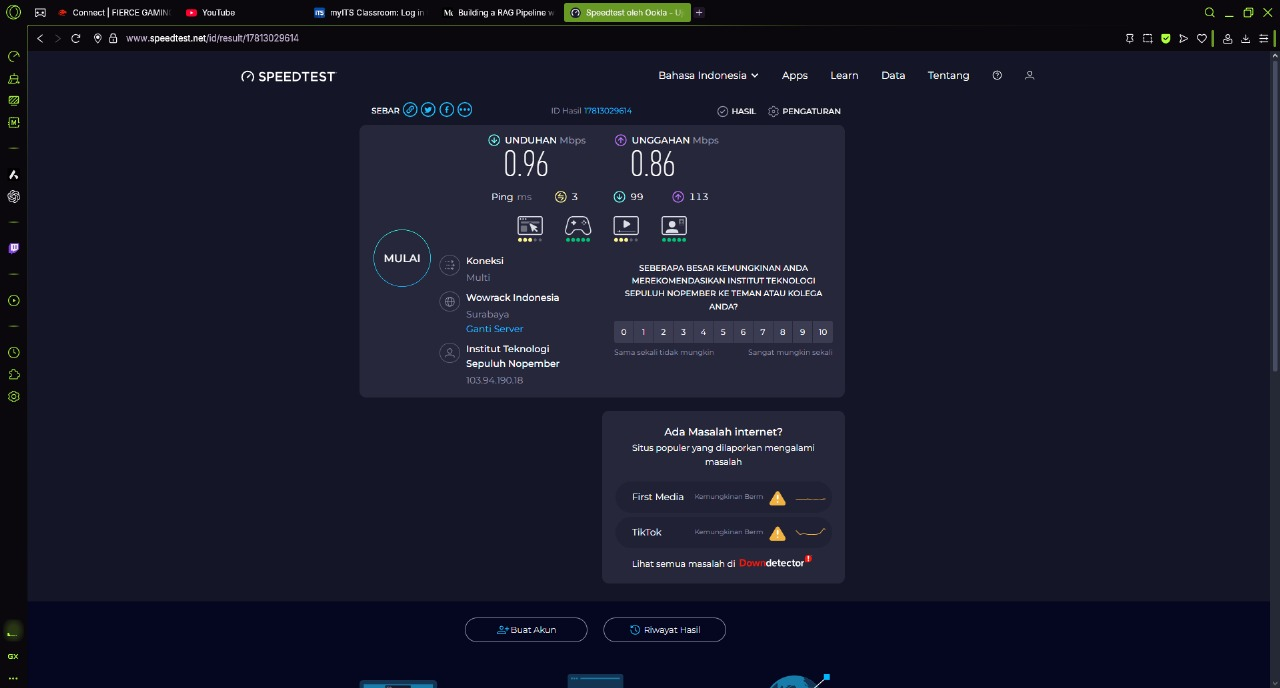
\includegraphics[width=\textwidth]{img5/Queuenonaktif.jpeg}
            \caption*{Speed test saat queue nonaktif}
        \end{minipage}\hfill
        \begin{minipage}{0.48\textwidth}
            \centering
            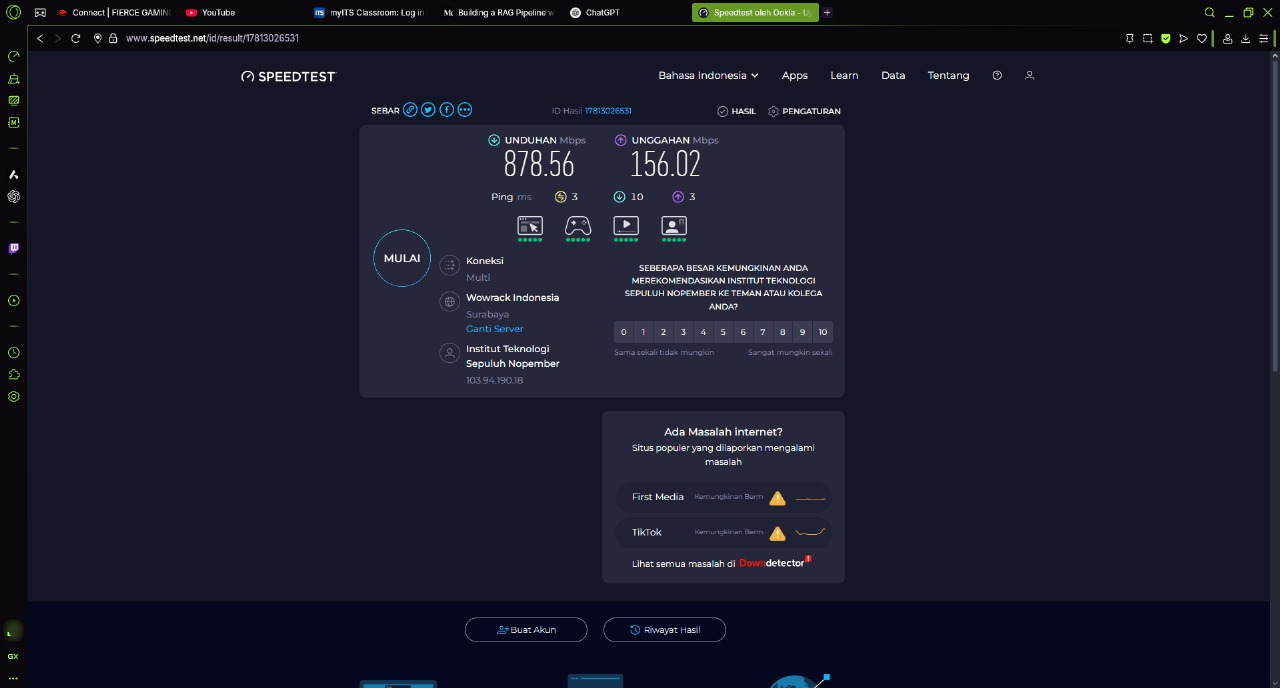
\includegraphics[width=\textwidth]{img5/Queueaktif.jpeg} 
            \caption*{Speed test saat queue aktif}
        \end{minipage}
        \captionof{figure}{Perbandingan hasil tes kecepatan internet sebelum dan sesudah Simple Queue diaktifkan.}
    \end{figure}
\end{enumerate}

\section{Analisis Hasil Percobaan}
\addcontentsline{toc}{section}{Analisis Hasil Percobaan}
Berdasarkan dua skenario praktikum yang telah saya lakukan pada router MikroTik, saya dapat menganalisis fungsionalitas dan relevansi dari setiap konfigurasi yang diterapkan.

\subsection*{$\bullet$ Analisis Konfigurasi VPN PPTP}
\addcontentsline{toc}{subsection}{Analisis Konfigurasi VPN PPTP}
Pada skenario pertama, saya berhasil membangun sebuah server VPN untuk koneksi \textit{remote access}. Proses ini menunjukkan beberapa poin penting. Pengaktifan \textbf{PPTP Server} pada router berfungsi sebagai "pendengar" yang siap menerima koneksi dari klien. Pembuatan kredensial pada tab \textbf{Secrets} adalah inti dari keamanan akses, di mana saya mendefinisikan username, password, serta alokasi alamat IP untuk klien yang akan terhubung.
Keberhasilan ping dari laptop klien (yang mendapat IP \texttt{192.168.10.5}) ke gateway router (\texttt{192.168.10.2}) dan ke PC lain di LAN membuktikan bahwa "terowongan" virtual telah terbentuk. Paket data dari laptop saya dibungkus menggunakan protokol PPTP, dikirim melalui internet, lalu dibuka kembali oleh router dan diteruskan ke jaringan lokal. Penggunaan \textbf{proxy-arp} pada antarmuka LAN juga krusial, karena memungkinkan router untuk "mewakili" klien VPN dalam komunikasi di jaringan lokal, sehingga seolah-olah klien VPN tersebut berada di segmen jaringan yang sama.

\subsection*{$\bullet$ Analisis Konfigurasi QoS dengan Simple Queue}
\addcontentsline{toc}{subsection}{Analisis Konfigurasi QoS dengan Simple Queue}
Pada skenario kedua, saya mengimplementasikan Quality of Service (QoS) untuk membatasi bandwidth. Saya menyimpulkan bahwa \textbf{Simple Queue} adalah metode yang sangat efektif dan mudah untuk manajemen bandwidth skala kecil hingga menengah. Dengan menargetkan seluruh subnet LAN (\texttt{192.168.10.0/24}), saya dapat menerapkan satu aturan untuk semua klien yang terhubung.
Pengaturan \textbf{Max Limit} ke \texttt{1M} terbukti berhasil membatasi kecepatan unduh dan unggah klien di sekitar 1 Mbps, seperti yang ditunjukkan oleh hasil perbandingan \textit{speed test}. Hal ini menunjukkan bahwa Simple Queue bekerja dengan cara memberlakukan batas atas (hard limit) pada lalu lintas yang cocok dengan target yang ditentukan. Fitur ini sangat relevan untuk lingkungan seperti jaringan kantor kecil atau publik di mana alokasi bandwidth yang adil dan terkontrol sangat diperlukan untuk menjaga stabilitas jaringan.

\newpage
\section{Tugas Modul}
\addcontentsline{toc}{section}{Tugas Modul}
Pada bagian ini, saya melakukan simulasi untuk membangun koneksi antar dua jaringan lokal yang terpisah menggunakan \textit{site-to-site tunnel} di Cisco Packet Tracer. Saya menggunakan GRE Tunnel sebagai metode implementasi yang paling lugas dan relevan secara konseptual.

\begin{enumerate}
    \item \textbf{Desain Topologi dan Pengalamatan IP:} Langkah pertama adalah merancang dan membangun topologi jaringan yang terdiri dari dua situs (diwakili PC dan Router) yang terhubung melalui router perantara (ISP). Skema pengalamatan IP yang terstruktur juga saya siapkan untuk memisahkan jaringan privat, publik, dan tunnel.
    \begin{center}
        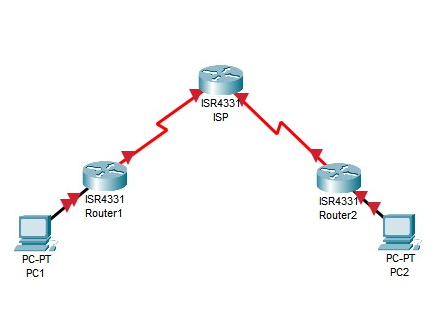
\includegraphics[width=0.7\textwidth]{img5/Topoawal.png}
        \captionof{figure}{Topologi jaringan site-to-site dengan 1 router ISP.}
    \end{center}

    \item \textbf{Konfigurasi IP Dasar dan Perkabelan:} Saya melakukan konfigurasi IP Address pada semua perangkat, termasuk PC klien dan semua antarmuka fisik router (LAN dan Serial). Sesuai praktik terbaik yang telah diperbaiki, saya memastikan sisi DCE dari koneksi serial menerima perintah \texttt{clock rate}.
    \begin{figure}[H]
        \centering
        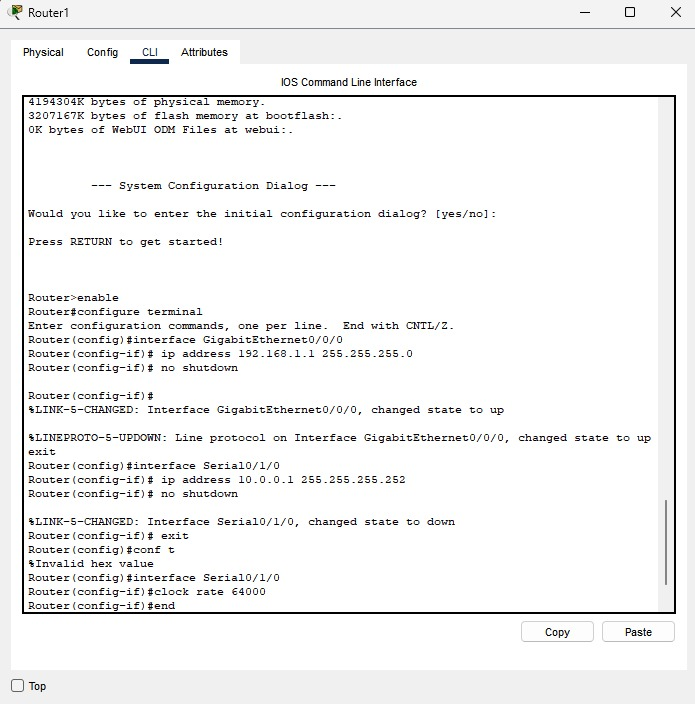
\includegraphics[width=0.8\textwidth]{img5/R1IPConf.jpeg}
        \captionof{figure}{Contoh konfigurasi IP Address pada salah satu router.}
    \end{figure}

    \item \textbf{Konfigurasi Routing Publik:} Agar router R1 dan R2 dapat berkomunikasi melalui ISP, saya menambahkan \textit{default route} di kedua router tersebut. Rute ini mengarahkan semua lalu lintas yang tidak dikenali ke router ISP, yang secara efektif menyediakan konektivitas "internet" dasar.
    \begin{center}
        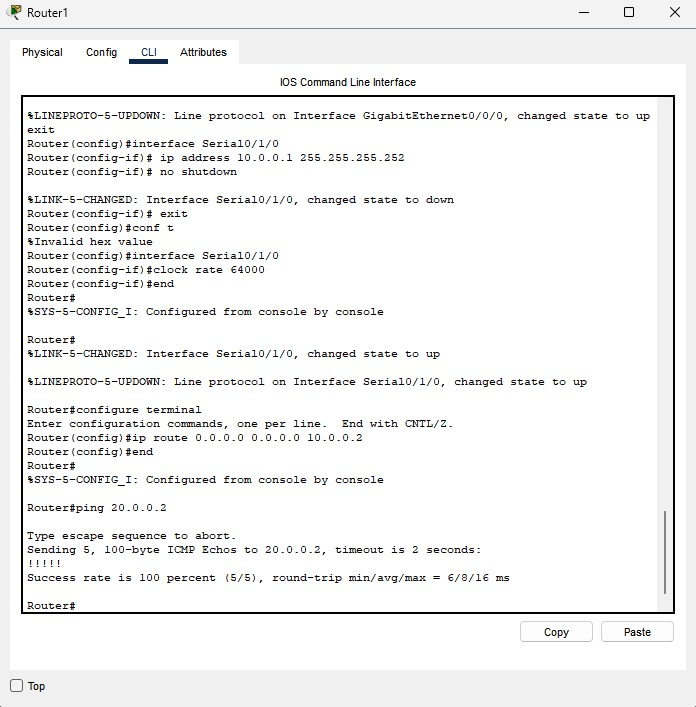
\includegraphics[width=0.7\textwidth]{img5/PingR1R2.jpeg}
        \captionof{figure}{Uji ping antar IP publik R1 dan R2 yang berhasil.}
    \end{center}

    \item \textbf{Pembangunan GRE Tunnel:} Ini adalah inti dari simulasi. Saya membuat antarmuka virtual \texttt{Tunnel0} di R1 dan R2. Konfigurasi \texttt{tunnel source} dan \texttt{tunnel destination} menggunakan alamat IP publik router, yang memerintahkan router untuk membungkus paket dan mengirimkannya melalui jaringan publik ke router tetangga.
    \begin{figure}[H]
        \centering
        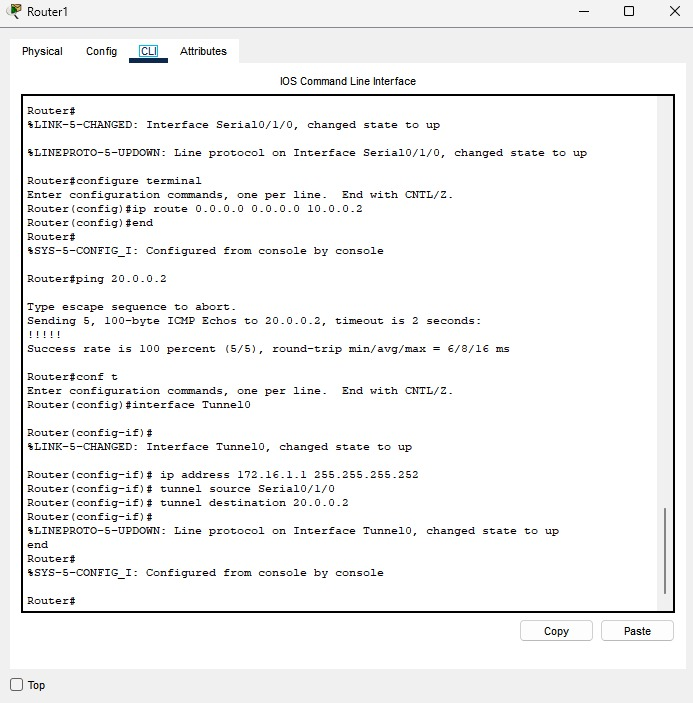
\includegraphics[width=0.7\textwidth]{img5/R1Tunnel.jpeg}
        \captionof{figure}{Konfigurasi antarmuka Tunnel0 pada R1.}
    \end{figure}
    
    \item \textbf{Verifikasi Konektivitas Tunnel:} Saya melakukan ping ke alamat IP tunnel dari router seberang. Keberhasilan ping ini mengonfirmasi bahwa "terowongan" virtual telah berhasil terbentuk dan aktif antara R1 dan R2.
    \begin{center}
        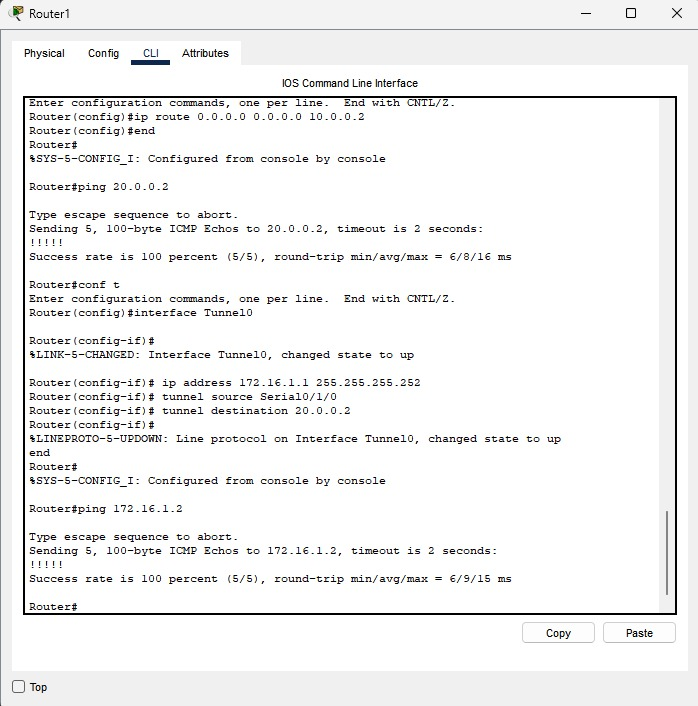
\includegraphics[width=0.6\textwidth]{img5/R1TunnelPing.jpeg}
        \captionof{figure}{Ping antar alamat IP tunnel (\texttt{172.16.1.1} dan \texttt{172.16.1.2}) berhasil.}
    \end{center}

    \item \textbf{Routing Statis Melalui Tunnel:} Setelah tunnel aktif, saya perlu mengarahkan lalu lintas antar-LAN untuk melewatinya. Ini dilakukan dengan menambahkan rute statis di R1 untuk menjangkau LAN-2 melalui IP tunnel R2, dan sebaliknya. Tanpa rute ini, paket dari PC1 ke PC2 akan dikirim ke internet via default route, bukan melalui tunnel.
    \begin{center}
        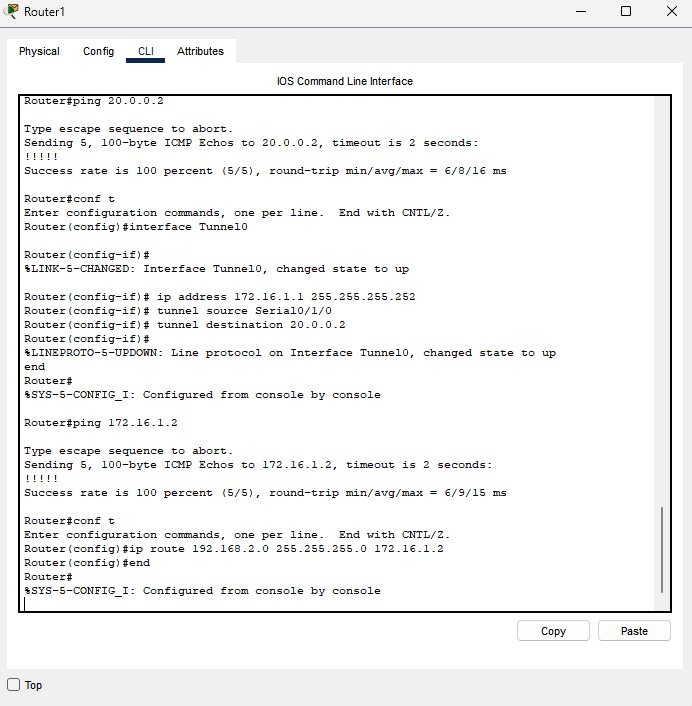
\includegraphics[width=0.8\textwidth]{img5/R1RouteStatic.jpeg}
        \captionof{figure}{Perintah rute statis untuk mengarahkan trafik LAN ke dalam tunnel.}
    \end{center}

    \item \textbf{Pengujian Akhir dan Verifikasi Jalur:} Sebagai pembuktian akhir, saya melakukan pengujian dari PC1 ke PC2.
    \begin{figure}[H]
        \centering
        \begin{minipage}{0.48\textwidth}
            \centering
            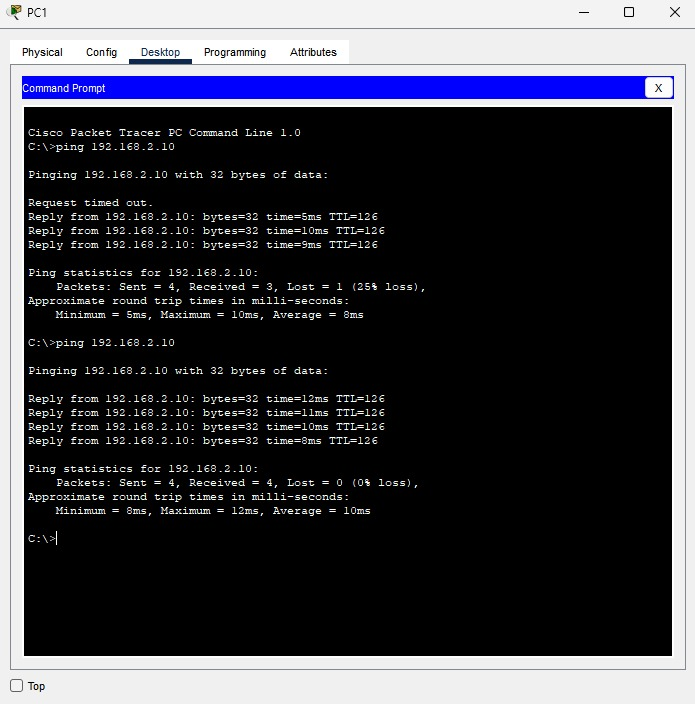
\includegraphics[width=\textwidth]{img5/Pingsuccess.jpeg}
            \caption*{(a) Hasil Ping Sukses}
        \end{minipage}\hfill
        \begin{minipage}{0.48\textwidth}
            \centering
            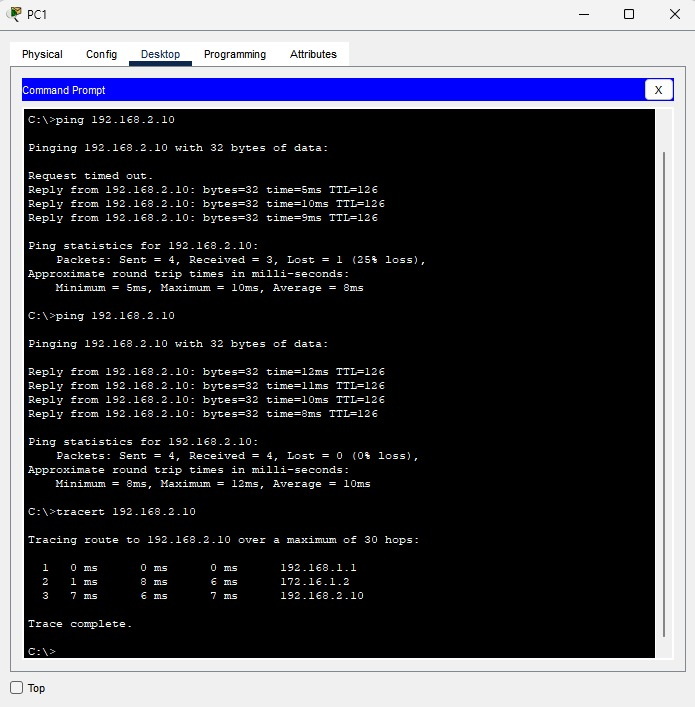
\includegraphics[width=\textwidth]{img5/P1Tracert.jpeg}
            \caption*{(b) Hasil Traceroute}
        \end{minipage}
        \captionof{figure}{Pengujian akhir menunjukkan (a) ping end-to-end berhasil dan (b) traceroute mengonfirmasi jalur melewati IP tunnel.}
    \end{figure}
\end{enumerate}

\section{Kesimpulan}
\addcontentsline{toc}{section}{Kesimpulan}

Praktikum modul kelima ini memberikan pemahaman yang utuh mengenai teknologi tunneling dan manajemen lalu lintas jaringan. Dari materi teori, saya memahami berbagai jenis protokol tunneling, dengan IPSec sebagai standar keamanan tinggi dan GRE sebagai metode enkapsulasi yang fleksibel. Pada praktikum MikroTik, saya berhasil menerapkan konsep ini secara nyata dengan membangun server VPN PPTP untuk skenario \textit{remote access}, yang membuktikan bagaimana sebuah "terowongan" logis dapat menghubungkan klien eksternal ke jaringan internal dengan aman. Selain itu, implementasi \textit{Simple Queue} memberikan pengalaman langsung dalam melakukan manajemen bandwidth, sebuah aspek krusial dari Quality of Service (QoS) untuk menjaga performa jaringan.

Selanjutnya, pada Tugas Modul, saya mengintegrasikan pengetahuan ini dalam skala yang berbeda melalui simulasi \textit{site-to-site tunnel}. Penggunaan GRE tunnel di Cisco Packet Tracer secara efektif mendemonstrasikan bagaimana dua jaringan privat yang terpisah dapat disatukan melalui jaringan publik. Proses ini menegaskan pentingnya routing berlapis: routing di jaringan fisik (dasar) untuk membentuk tunnel, dan routing di atas tunnel (overlay) untuk melewatkan data pengguna. Secara keseluruhan, saya menyimpulkan bahwa teknologi tunneling dan QoS adalah pilar fundamental dalam rekayasa jaringan modern, yang masing-masing berfungsi untuk menyediakan konektivitas yang aman dan terukur melintasi batas-batas jaringan fisik.

\section{Lampiran}
\subsection*{Dokumentasi saat praktikum}
\addcontentsline{toc}{subsection}{Dokumentasi saat praktikum}
Berikut adalah dokumentasi saat praktikum Modul 4 berlangsung.

\begin{figure}[H]
    \centering
    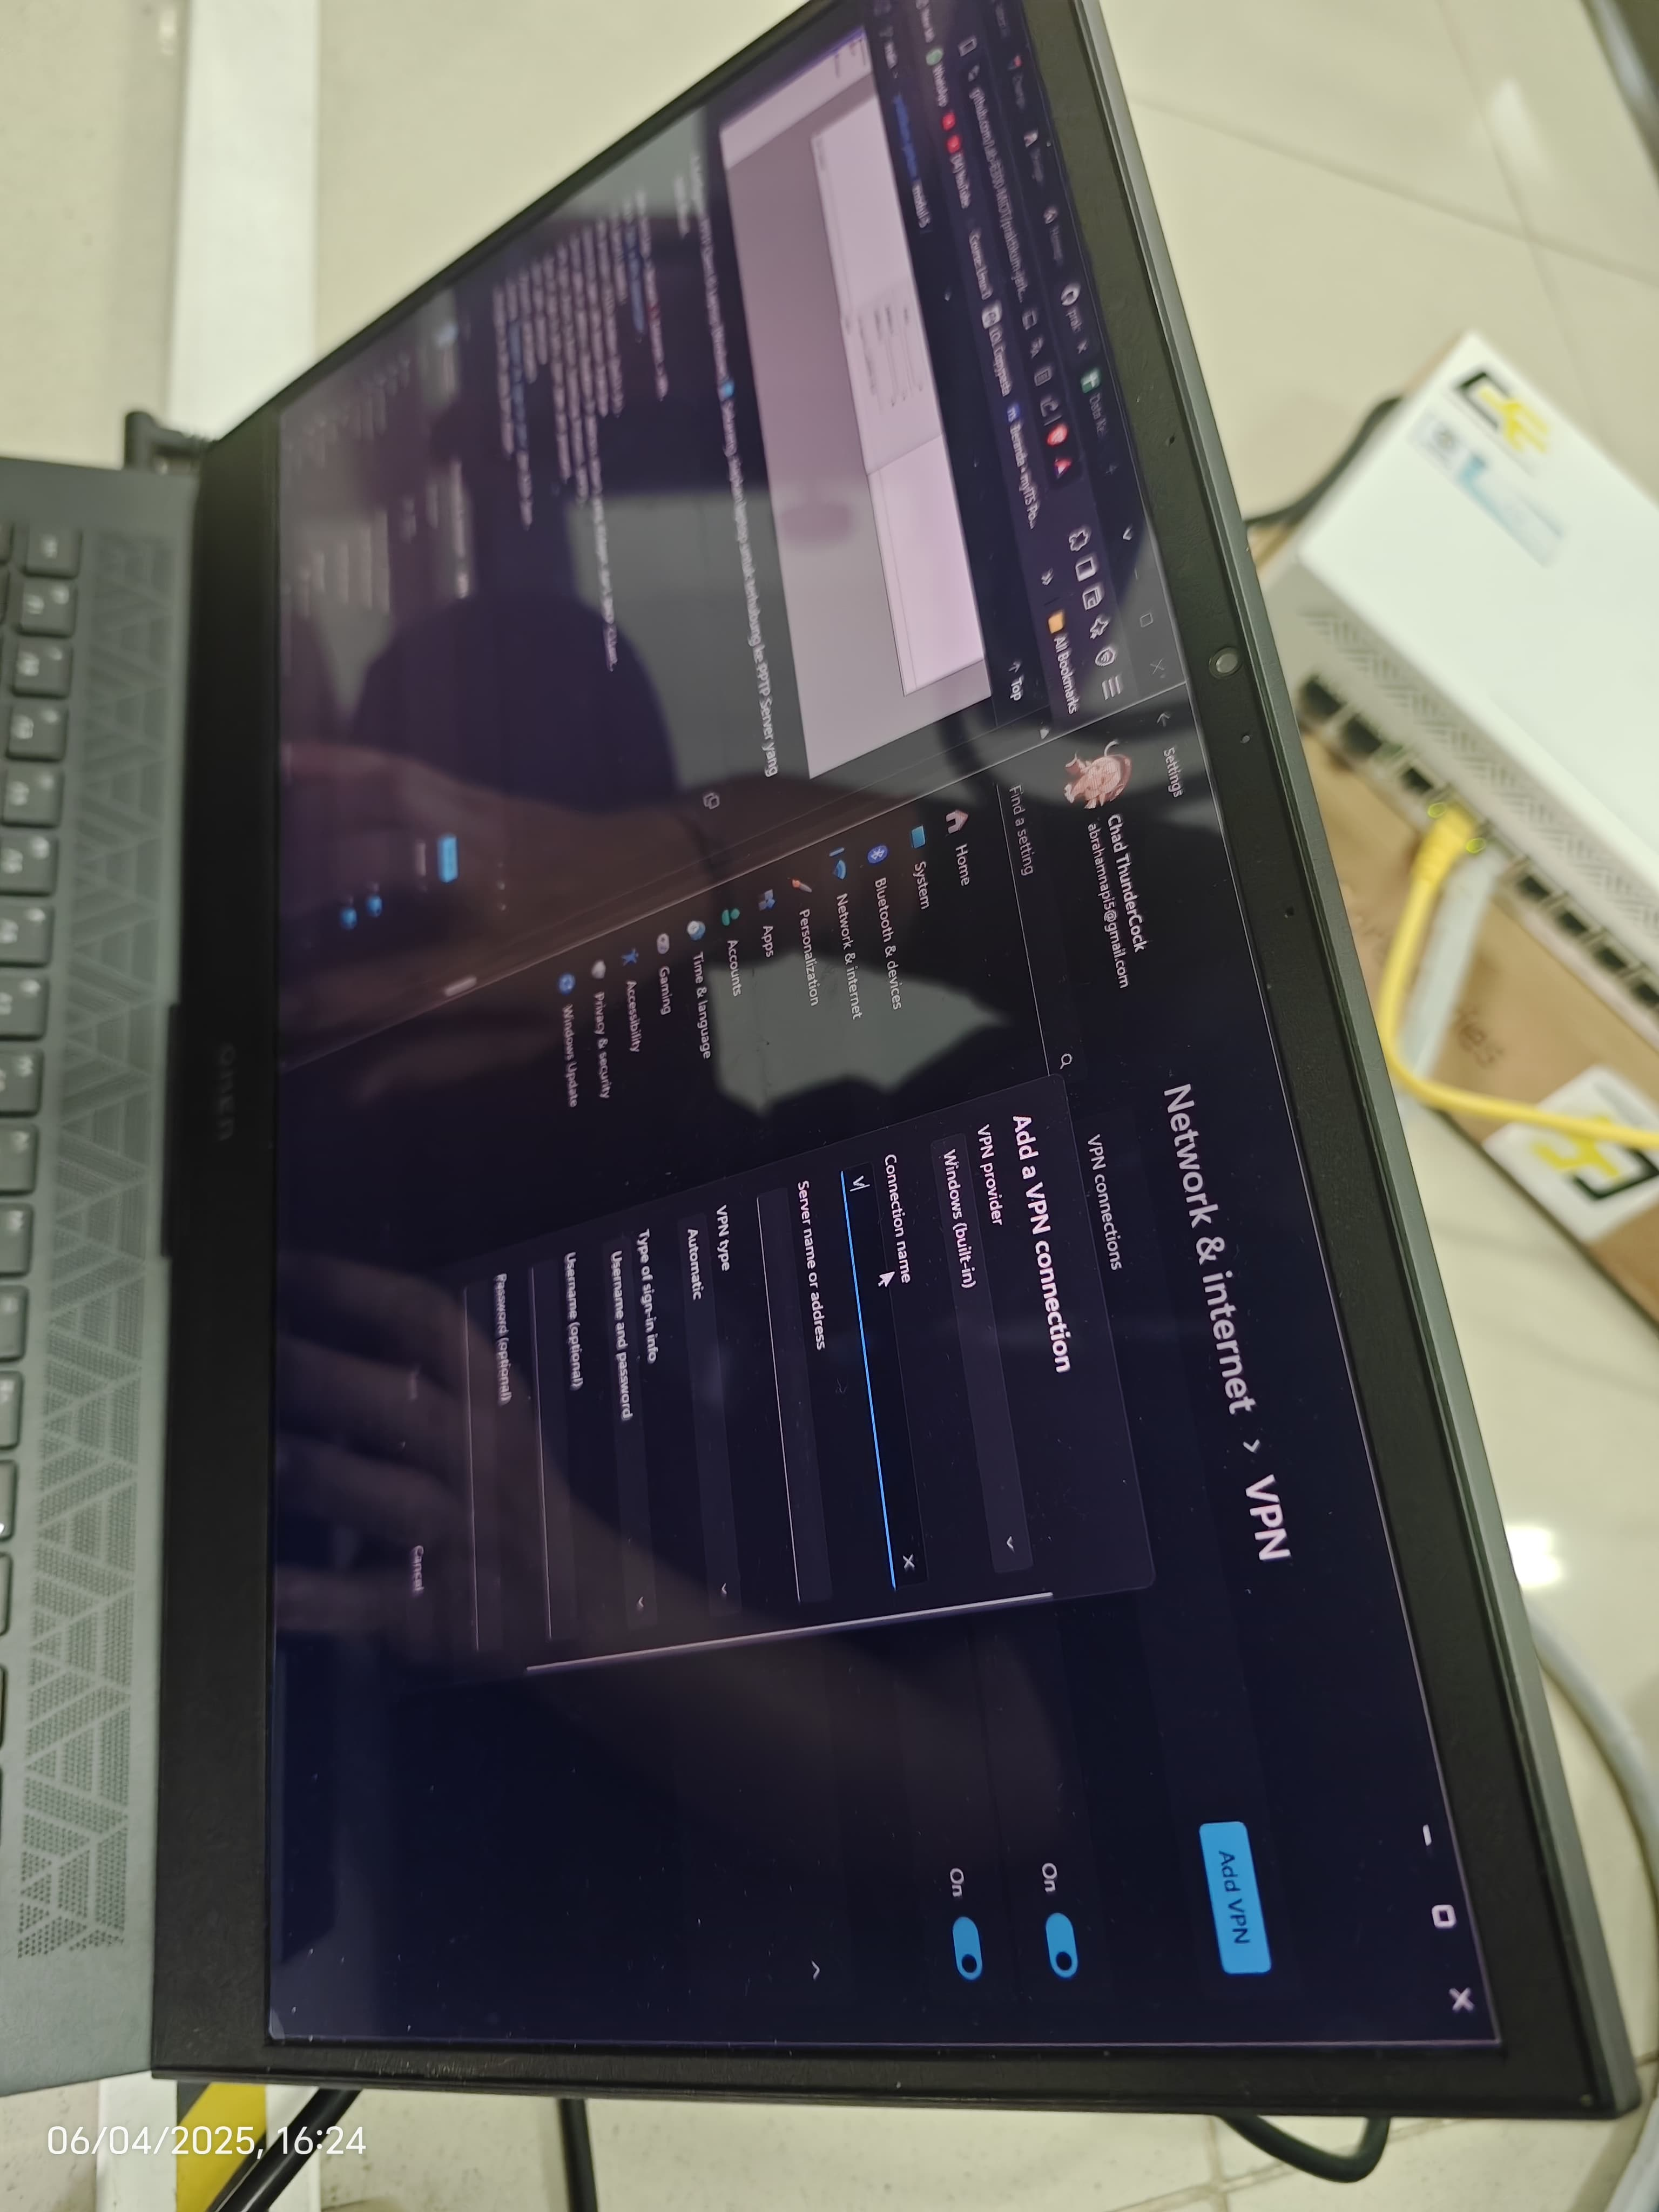
\includegraphics[width=0.7\textwidth]{img5/lampiran5.jpeg} 
    \caption{Dokumentasi praktikum.}
\end{figure}

\end{document}

\end{document}